\documentclass{standalone}
\usepackage{tikz}
\usetikzlibrary{patterns, positioning}


\begin{document}
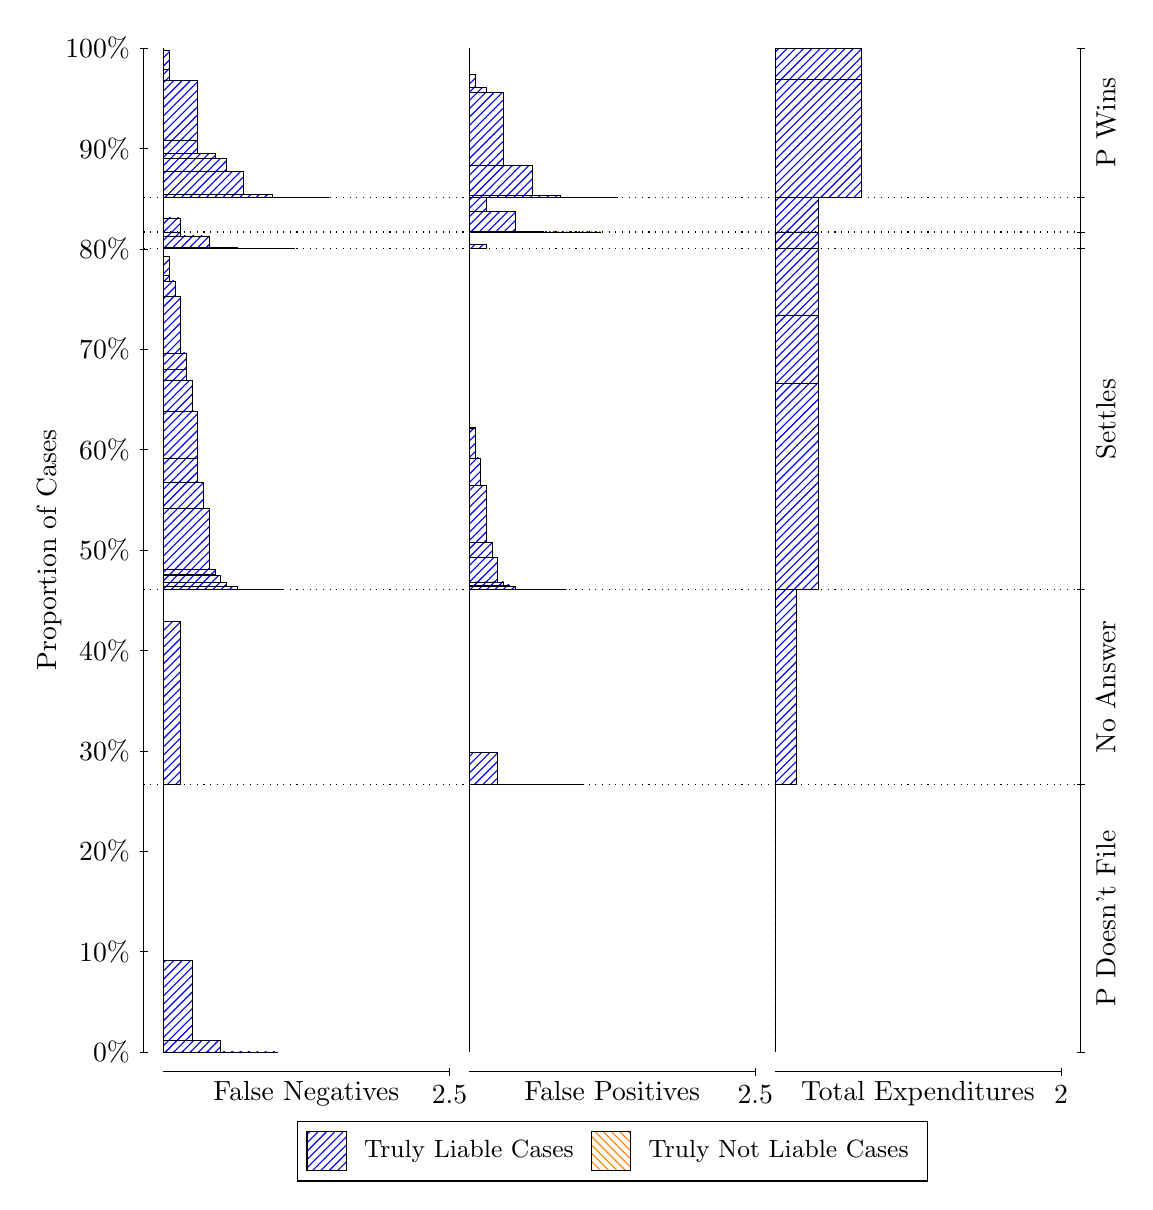
\begin{tikzpicture}
\draw[black, very thin] (1.5,1.75) -- (1.5,14.5);
\node[rotate=90, text=black, anchor=center] at (0.3, 8.125) {Proportion of Cases};
\draw[black, very thin] (1.45,1.75) -- (1.55,1.75);
\node[text=black, anchor=east] at (1.45, 1.75) {0\%};
\draw[black, very thin] (1.45,3.025) -- (1.55,3.025);
\node[text=black, anchor=east] at (1.45, 3.025) {10\%};
\draw[black, very thin] (1.45,4.3) -- (1.55,4.3);
\node[text=black, anchor=east] at (1.45, 4.3) {20\%};
\draw[black, very thin] (1.45,5.575) -- (1.55,5.575);
\node[text=black, anchor=east] at (1.45, 5.575) {30\%};
\draw[black, very thin] (1.45,6.85) -- (1.55,6.85);
\node[text=black, anchor=east] at (1.45, 6.85) {40\%};
\draw[black, very thin] (1.45,8.125) -- (1.55,8.125);
\node[text=black, anchor=east] at (1.45, 8.125) {50\%};
\draw[black, very thin] (1.45,9.4) -- (1.55,9.4);
\node[text=black, anchor=east] at (1.45, 9.4) {60\%};
\draw[black, very thin] (1.45,10.675) -- (1.55,10.675);
\node[text=black, anchor=east] at (1.45, 10.675) {70\%};
\draw[black, very thin] (1.45,11.95) -- (1.55,11.95);
\node[text=black, anchor=east] at (1.45, 11.95) {80\%};
\draw[black, very thin] (1.45,13.225) -- (1.55,13.225);
\node[text=black, anchor=east] at (1.45, 13.225) {90\%};
\draw[black, very thin] (1.45,14.5) -- (1.55,14.5);
\node[text=black, anchor=east] at (1.45, 14.5) {100\%};

\draw[black, very thin] (13.4,1.75) -- (13.4,14.5);
\draw[black, very thin] (13.35,1.75) -- (13.45,1.75);
\node[anchor=west] at (13.35, 1.75) {};
\draw[black, very thin] (13.35,5.1469) -- (13.45,5.1469);
\node[anchor=west] at (13.35, 5.1469) {};
\draw[black, very thin] (13.35,7.6207) -- (13.45,7.6207);
\node[anchor=west] at (13.35, 7.6207) {};
\draw[black, very thin] (13.35,11.954) -- (13.45,11.954);
\node[anchor=west] at (13.35, 11.954) {};
\draw[black, very thin] (13.35,12.164) -- (13.45,12.164);
\node[anchor=west] at (13.35, 12.164) {};
\draw[black, very thin] (13.35,12.603) -- (13.45,12.603);
\node[anchor=west] at (13.35, 12.603) {};
\draw[black, very thin] (13.35,14.5) -- (13.45,14.5);
\node[anchor=west] at (13.35, 14.5) {};

\draw[black, very thin, pattern color=blue, pattern=north east lines] (1.75,1.75) rectangle (3.2033,1.75);
\draw[black, very thin, pattern color=blue, pattern=north east lines] (1.75,1.75) rectangle (2.84,1.7512);
\draw[black, very thin, pattern color=blue, pattern=north east lines] (1.75,1.7512) rectangle (2.4767,1.8957);
\draw[black, very thin, pattern color=blue, pattern=north east lines] (1.75,1.8957) rectangle (2.1133,2.9102);
\draw[black, very thin, pattern color=orange, pattern=north west lines] (1.75,2.9102) rectangle (1.75,2.9102);
\draw[black, very thin, pattern color=blue, pattern=north east lines] (1.75,2.9102) rectangle (1.75,5.1469);
\draw[black, very thin, pattern color=blue, pattern=north east lines] (1.75,5.1469) rectangle (1.968,7.216);
\draw[black, very thin, pattern color=orange, pattern=north west lines] (1.75,7.216) rectangle (1.75,7.216);
\draw[black, very thin, pattern color=blue, pattern=north east lines] (1.75,7.216) rectangle (1.75,7.6207);
\draw[black, very thin, pattern color=blue, pattern=north east lines] (1.75,7.6207) rectangle (3.276,7.6207);
\draw[black, very thin, pattern color=blue, pattern=north east lines] (1.75,7.6207) rectangle (3.1307,7.6207);
\draw[black, very thin, pattern color=blue, pattern=north east lines] (1.75,7.6207) rectangle (2.9853,7.6207);
\draw[black, very thin, pattern color=blue, pattern=north east lines] (1.75,7.6207) rectangle (2.9127,7.6207);
\draw[black, very thin, pattern color=blue, pattern=north east lines] (1.75,7.6207) rectangle (2.84,7.6209);
\draw[black, very thin, pattern color=blue, pattern=north east lines] (1.75,7.6209) rectangle (2.7673,7.6211);
\draw[black, very thin, pattern color=blue, pattern=north east lines] (1.75,7.6211) rectangle (2.6947,7.6591);
\draw[black, very thin, pattern color=blue, pattern=north east lines] (1.75,7.6591) rectangle (2.622,7.6703);
\draw[black, very thin, pattern color=blue, pattern=north east lines] (1.75,7.6703) rectangle (2.5493,7.7132);
\draw[black, very thin, pattern color=blue, pattern=north east lines] (1.75,7.7132) rectangle (2.4767,7.8021);
\draw[black, very thin, pattern color=blue, pattern=north east lines] (1.75,7.8021) rectangle (2.404,7.8121);
\draw[black, very thin, pattern color=blue, pattern=north east lines] (1.75,7.8121) rectangle (2.404,7.8795);
\draw[black, very thin, pattern color=blue, pattern=north east lines] (1.75,7.8795) rectangle (2.3313,8.6516);
\draw[black, very thin, pattern color=blue, pattern=north east lines] (1.75,8.6516) rectangle (2.2587,8.9895);
\draw[black, very thin, pattern color=blue, pattern=north east lines] (1.75,8.9895) rectangle (2.186,9.294);
\draw[black, very thin, pattern color=blue, pattern=north east lines] (1.75,9.294) rectangle (2.186,9.8908);
\draw[black, very thin, pattern color=blue, pattern=north east lines] (1.75,9.8908) rectangle (2.1133,10.281);
\draw[black, very thin, pattern color=blue, pattern=north east lines] (1.75,10.281) rectangle (2.0407,10.414);
\draw[black, very thin, pattern color=blue, pattern=north east lines] (1.75,10.414) rectangle (2.0407,10.628);
\draw[black, very thin, pattern color=blue, pattern=north east lines] (1.75,10.628) rectangle (1.968,11.349);
\draw[black, very thin, pattern color=blue, pattern=north east lines] (1.75,11.349) rectangle (1.8953,11.542);
\draw[black, very thin, pattern color=blue, pattern=north east lines] (1.75,11.542) rectangle (1.8227,11.61);
\draw[black, very thin, pattern color=blue, pattern=north east lines] (1.75,11.61) rectangle (1.8227,11.853);
\draw[black, very thin, pattern color=blue, pattern=north east lines] (1.75,11.853) rectangle (1.75,11.854);
\draw[black, very thin, pattern color=orange, pattern=north west lines] (1.75,11.854) rectangle (1.75,11.854);
\draw[black, very thin, pattern color=blue, pattern=north east lines] (1.75,11.854) rectangle (1.75,11.954);
\draw[black, very thin, pattern color=blue, pattern=north east lines] (1.75,11.954) rectangle (3.4213,11.954);
\draw[black, very thin, pattern color=blue, pattern=north east lines] (1.75,11.954) rectangle (3.058,11.954);
\draw[black, very thin, pattern color=blue, pattern=north east lines] (1.75,11.954) rectangle (2.6947,11.971);
\draw[black, very thin, pattern color=blue, pattern=north east lines] (1.75,11.971) rectangle (2.3313,12.115);
\draw[black, very thin, pattern color=blue, pattern=north east lines] (1.75,12.115) rectangle (1.968,12.164);
\draw[black, very thin, pattern color=orange, pattern=north west lines] (1.75,12.164) rectangle (1.75,12.164);
\draw[black, very thin, pattern color=blue, pattern=north east lines] (1.75,12.164) rectangle (1.968,12.342);
\draw[black, very thin, pattern color=orange, pattern=north west lines] (1.75,12.342) rectangle (1.75,12.342);
\draw[black, very thin, pattern color=blue, pattern=north east lines] (1.75,12.342) rectangle (1.75,12.603);
\draw[black, very thin, pattern color=blue, pattern=north east lines] (1.75,12.603) rectangle (3.8573,12.603);
\draw[black, very thin, pattern color=blue, pattern=north east lines] (1.75,12.603) rectangle (3.494,12.603);
\draw[black, very thin, pattern color=blue, pattern=north east lines] (1.75,12.603) rectangle (3.276,12.603);
\draw[black, very thin, pattern color=blue, pattern=north east lines] (1.75,12.603) rectangle (3.1307,12.641);
\draw[black, very thin, pattern color=blue, pattern=north east lines] (1.75,12.641) rectangle (2.9127,12.641);
\draw[black, very thin, pattern color=blue, pattern=north east lines] (1.75,12.641) rectangle (2.7673,12.936);
\draw[black, very thin, pattern color=blue, pattern=north east lines] (1.75,12.936) rectangle (2.5493,13.099);
\draw[black, very thin, pattern color=blue, pattern=north east lines] (1.75,13.099) rectangle (2.404,13.166);
\draw[black, very thin, pattern color=blue, pattern=north east lines] (1.75,13.166) rectangle (2.186,13.323);
\draw[black, very thin, pattern color=blue, pattern=north east lines] (1.75,13.323) rectangle (2.186,14.089);
\draw[black, very thin, pattern color=blue, pattern=north east lines] (1.75,14.089) rectangle (2.0407,14.089);
\draw[black, very thin, pattern color=blue, pattern=north east lines] (1.75,14.089) rectangle (1.8227,14.226);
\draw[black, very thin, pattern color=blue, pattern=north east lines] (1.75,14.226) rectangle (1.8227,14.476);
\draw[black, very thin, pattern color=orange, pattern=north west lines] (1.75,14.476) rectangle (1.75,14.476);
\draw[black, very thin, pattern color=blue, pattern=north east lines] (1.75,14.476) rectangle (1.75,14.5);
\draw[black, very thin, pattern color=orange, pattern=north west lines] (5.6333,1.75) rectangle (5.6333,1.75);
\draw[black, very thin, pattern color=blue, pattern=north east lines] (5.6333,1.75) rectangle (5.6333,5.1469);
\draw[black, very thin, pattern color=orange, pattern=north west lines] (5.6333,5.1469) rectangle (7.0867,5.1469);
\draw[black, very thin, pattern color=blue, pattern=north east lines] (5.6333,5.1469) rectangle (7.0867,5.1469);
\draw[black, very thin, pattern color=blue, pattern=north east lines] (5.6333,5.1469) rectangle (6.7233,5.1469);
\draw[black, very thin, pattern color=blue, pattern=north east lines] (5.6333,5.1469) rectangle (6.36,5.1502);
\draw[black, very thin, pattern color=blue, pattern=north east lines] (5.6333,5.1502) rectangle (5.9967,5.5517);
\draw[black, very thin, pattern color=blue, pattern=north east lines] (5.6333,5.5517) rectangle (5.6333,7.6207);
\draw[black, very thin, pattern color=orange, pattern=north west lines] (5.6333,7.6207) rectangle (6.8687,7.6207);
\draw[black, very thin, pattern color=blue, pattern=north east lines] (5.6333,7.6207) rectangle (6.8687,7.6207);
\draw[black, very thin, pattern color=orange, pattern=north west lines] (5.6333,7.6207) rectangle (6.7233,7.6207);
\draw[black, very thin, pattern color=blue, pattern=north east lines] (5.6333,7.6207) rectangle (6.7233,7.6207);
\draw[black, very thin, pattern color=orange, pattern=north west lines] (5.6333,7.6207) rectangle (6.578,7.6207);
\draw[black, very thin, pattern color=blue, pattern=north east lines] (5.6333,7.6207) rectangle (6.578,7.6209);
\draw[black, very thin, pattern color=blue, pattern=north east lines] (5.6333,7.6209) rectangle (6.5053,7.6209);
\draw[black, very thin, pattern color=orange, pattern=north west lines] (5.6333,7.6209) rectangle (6.4327,7.6209);
\draw[black, very thin, pattern color=blue, pattern=north east lines] (5.6333,7.6209) rectangle (6.4327,7.6213);
\draw[black, very thin, pattern color=orange, pattern=north west lines] (5.6333,7.6213) rectangle (6.4327,7.6213);
\draw[black, very thin, pattern color=blue, pattern=north east lines] (5.6333,7.6213) rectangle (6.4327,7.6213);
\draw[black, very thin, pattern color=blue, pattern=north east lines] (5.6333,7.6213) rectangle (6.36,7.6214);
\draw[black, very thin, pattern color=orange, pattern=north west lines] (5.6333,7.6214) rectangle (6.2873,7.6214);
\draw[black, very thin, pattern color=blue, pattern=north east lines] (5.6333,7.6214) rectangle (6.2873,7.6262);
\draw[black, very thin, pattern color=blue, pattern=north east lines] (5.6333,7.6262) rectangle (6.2147,7.664);
\draw[black, very thin, pattern color=orange, pattern=north west lines] (5.6333,7.664) rectangle (6.142,7.664);
\draw[black, very thin, pattern color=blue, pattern=north east lines] (5.6333,7.664) rectangle (6.142,7.6831);
\draw[black, very thin, pattern color=blue, pattern=north east lines] (5.6333,7.6831) rectangle (6.0693,7.7207);
\draw[black, very thin, pattern color=blue, pattern=north east lines] (5.6333,7.7207) rectangle (6.0693,7.7211);
\draw[black, very thin, pattern color=orange, pattern=north west lines] (5.6333,7.7211) rectangle (5.9967,7.7211);
\draw[black, very thin, pattern color=blue, pattern=north east lines] (5.6333,7.7211) rectangle (5.9967,8.0323);
\draw[black, very thin, pattern color=blue, pattern=north east lines] (5.6333,8.0323) rectangle (5.924,8.2254);
\draw[black, very thin, pattern color=blue, pattern=north east lines] (5.6333,8.2254) rectangle (5.8513,8.9467);
\draw[black, very thin, pattern color=blue, pattern=north east lines] (5.6333,8.9467) rectangle (5.7787,9.2938);
\draw[black, very thin, pattern color=blue, pattern=north east lines] (5.6333,9.2938) rectangle (5.706,9.6722);
\draw[black, very thin, pattern color=blue, pattern=north east lines] (5.6333,9.6722) rectangle (5.706,9.6836);
\draw[black, very thin, pattern color=blue, pattern=north east lines] (5.6333,9.6836) rectangle (5.6333,11.954);
\draw[black, very thin, pattern color=orange, pattern=north west lines] (5.6333,11.954) rectangle (5.8513,11.954);
\draw[black, very thin, pattern color=blue, pattern=north east lines] (5.6333,11.954) rectangle (5.8513,12.003);
\draw[black, very thin, pattern color=blue, pattern=north east lines] (5.6333,12.003) rectangle (5.6333,12.164);
\draw[black, very thin, pattern color=orange, pattern=north west lines] (5.6333,12.164) rectangle (7.3047,12.164);
\draw[black, very thin, pattern color=blue, pattern=north east lines] (5.6333,12.164) rectangle (7.3047,12.164);
\draw[black, very thin, pattern color=blue, pattern=north east lines] (5.6333,12.164) rectangle (6.9413,12.164);
\draw[black, very thin, pattern color=blue, pattern=north east lines] (5.6333,12.164) rectangle (6.578,12.172);
\draw[black, very thin, pattern color=blue, pattern=north east lines] (5.6333,12.172) rectangle (6.2147,12.425);
\draw[black, very thin, pattern color=blue, pattern=north east lines] (5.6333,12.425) rectangle (5.8513,12.603);
\draw[black, very thin, pattern color=orange, pattern=north west lines] (5.6333,12.603) rectangle (7.5227,12.603);
\draw[black, very thin, pattern color=blue, pattern=north east lines] (5.6333,12.603) rectangle (7.5227,12.603);
\draw[black, very thin, pattern color=orange, pattern=north west lines] (5.6333,12.603) rectangle (7.1593,12.603);
\draw[black, very thin, pattern color=blue, pattern=north east lines] (5.6333,12.603) rectangle (7.1593,12.603);
\draw[black, very thin, pattern color=orange, pattern=north west lines] (5.6333,12.603) rectangle (6.796,12.603);
\draw[black, very thin, pattern color=blue, pattern=north east lines] (5.6333,12.603) rectangle (6.796,12.627);
\draw[black, very thin, pattern color=orange, pattern=north west lines] (5.6333,12.627) rectangle (6.578,12.627);
\draw[black, very thin, pattern color=blue, pattern=north east lines] (5.6333,12.627) rectangle (6.578,12.627);
\draw[black, very thin, pattern color=orange, pattern=north west lines] (5.6333,12.627) rectangle (6.4327,12.627);
\draw[black, very thin, pattern color=blue, pattern=north east lines] (5.6333,12.627) rectangle (6.4327,13.014);
\draw[black, very thin, pattern color=orange, pattern=north west lines] (5.6333,13.014) rectangle (6.2147,13.014);
\draw[black, very thin, pattern color=blue, pattern=north east lines] (5.6333,13.014) rectangle (6.2147,13.014);
\draw[black, very thin, pattern color=blue, pattern=north east lines] (5.6333,13.014) rectangle (6.0693,13.937);
\draw[black, very thin, pattern color=blue, pattern=north east lines] (5.6333,13.937) rectangle (5.8513,14.001);
\draw[black, very thin, pattern color=orange, pattern=north west lines] (5.6333,14.001) rectangle (5.8513,14.001);
\draw[black, very thin, pattern color=blue, pattern=north east lines] (5.6333,14.001) rectangle (5.8513,14.004);
\draw[black, very thin, pattern color=blue, pattern=north east lines] (5.6333,14.004) rectangle (5.706,14.167);
\draw[black, very thin, pattern color=blue, pattern=north east lines] (5.6333,14.167) rectangle (5.6333,14.5);
\draw[black, very thin, pattern color=orange, pattern=north west lines] (9.5167,1.75) rectangle (9.5167,1.75);
\draw[black, very thin, pattern color=blue, pattern=north east lines] (9.5167,1.75) rectangle (9.5167,5.1469);
\draw[black, very thin, pattern color=orange, pattern=north west lines] (9.5167,5.1469) rectangle (9.7892,5.1469);
\draw[black, very thin, pattern color=blue, pattern=north east lines] (9.5167,5.1469) rectangle (9.7892,7.6207);
\draw[black, very thin, pattern color=orange, pattern=north west lines] (9.5167,7.6207) rectangle (10.062,7.6207);
\draw[black, very thin, pattern color=blue, pattern=north east lines] (9.5167,7.6207) rectangle (10.062,10.238);
\draw[black, very thin, pattern color=orange, pattern=north west lines] (9.5167,10.238) rectangle (10.062,10.238);
\draw[black, very thin, pattern color=blue, pattern=north east lines] (9.5167,10.238) rectangle (10.062,11.101);
\draw[black, very thin, pattern color=orange, pattern=north west lines] (9.5167,11.101) rectangle (10.062,11.101);
\draw[black, very thin, pattern color=blue, pattern=north east lines] (9.5167,11.101) rectangle (10.062,11.954);
\draw[black, very thin, pattern color=orange, pattern=north west lines] (9.5167,11.954) rectangle (10.062,11.954);
\draw[black, very thin, pattern color=blue, pattern=north east lines] (9.5167,11.954) rectangle (10.062,12.164);
\draw[black, very thin, pattern color=orange, pattern=north west lines] (9.5167,12.164) rectangle (10.062,12.164);
\draw[black, very thin, pattern color=blue, pattern=north east lines] (9.5167,12.164) rectangle (10.062,12.603);
\draw[black, very thin, pattern color=orange, pattern=north west lines] (9.5167,12.603) rectangle (10.607,12.603);
\draw[black, very thin, pattern color=blue, pattern=north east lines] (9.5167,12.603) rectangle (10.607,14.1);
\draw[black, very thin, pattern color=orange, pattern=north west lines] (9.5167,14.1) rectangle (10.607,14.1);
\draw[black, very thin, pattern color=blue, pattern=north east lines] (9.5167,14.1) rectangle (10.607,14.5);
\draw[black, dotted] (1.5,5.1469) -- (13.4,5.1469);
\draw[black, dotted] (1.5,7.6207) -- (13.4,7.6207);
\draw[black, dotted] (1.5,11.954) -- (13.4,11.954);
\draw[black, dotted] (1.5,12.164) -- (13.4,12.164);
\draw[black, dotted] (1.5,12.603) -- (13.4,12.603);
\draw[black, very thin] (1.75,1.5) -- (5.3833,1.5);
\node[text=black, anchor=north] at (3.5667, 1.5) {False Negatives};
\draw[black, very thin] (5.3833,1.45) -- (5.3833,1.55);
\node[text=black, anchor=north] at (5.3833, 1.45) {2.5};

\draw[black, very thin] (5.6333,1.5) -- (9.2667,1.5);
\node[text=black, anchor=north] at (7.45, 1.5) {False Positives};
\draw[black, very thin] (9.2667,1.45) -- (9.2667,1.55);
\node[text=black, anchor=north] at (9.2667, 1.45) {2.5};

\draw[black, very thin] (9.5167,1.5) -- (13.15,1.5);
\node[text=black, anchor=north] at (11.333, 1.5) {Total Expenditures};
\draw[black, very thin] (13.15,1.45) -- (13.15,1.55);
\node[text=black, anchor=north] at (13.15, 1.45) {2};

\node[text=black, centered, rotate=90] at (13.72, 3.4485) {P Doesn't File};
\node[text=black, centered, rotate=90] at (13.72, 6.3838) {No Answer};
\node[text=black, centered, rotate=90] at (13.72, 9.7872) {Settles};


\node[text=black, centered, rotate=90] at (13.72, 13.552) {P Wins};

\draw (7.449999999999999,1.5) node[draw=none] (baseCoordinate) {};
\begin{scope}[align=center]
        \matrix[scale=0.5, draw=black, below=0.5cm of baseCoordinate, nodes={draw}, column sep=0.1cm]{
            \node[rectangle, draw, minimum width=0.5cm, minimum height=0.5cm, pattern color=blue, pattern=north east lines] {}; &
            \node[draw=none, font=\small, text=black] (B) {Truly Liable Cases}; &
            \node[rectangle, draw, minimum width=0.5cm, minimum height=0.5cm, pattern color=orange, pattern=north west lines] {}; &
            \node[draw=none, font=\small, text=black] (B) {Truly Not Liable Cases}; \\
            };
\end{scope}

\end{tikzpicture}
\end{document}